
\chapter{Einleitung}
\label{ch: Einleitung}
	
	\section{Motivation}
	\label{sec: Motivation}
		Das Thema der künstlichen Intelligenz (KI) ist heutzutage allgegenwärtig. Smart Home Geräte wie Amazons Alexa, Siri der Firma Apple oder der Google Assistant gehören mittlerweile in jeden ... deutschen Haushalt und enthalten KI zur Spracherkennung. Derartige Technologien begleiten den Menschen jedoch nicht nur Zuhause sondern auch in der Transport- und Logistikbranche. Eine Potenzialanalyse zur künstlichen Intelligenz der Firma Sopra Steria zeigt, dass bereits im Jahr 2017 20\% aller befragten Unternehmen solche Systeme einsetzten. 37\% planten den zukünftigen Einsatz. Die Implementierung solcher Systeme hat Einfluss auf verschiedenste Eigenschaften der Wertschöpfungskette. Die Qualität des Fachprozesses wird mit ebenfalls steigender Geschwindigkeit erhöht. Die zur Logistikbranche gehörenden Transportfahrzeuge sind ebenfalls mit KI ausgestattet und sorgen so für weniger Arbeitsunfälle und eine schnellere, präzisiere Abarbeitung der Logistikaufgaben.\\
		
		\begin{figure}[H]
			\begin{minipage}[b]{0.49\textwidth}
				(a)
				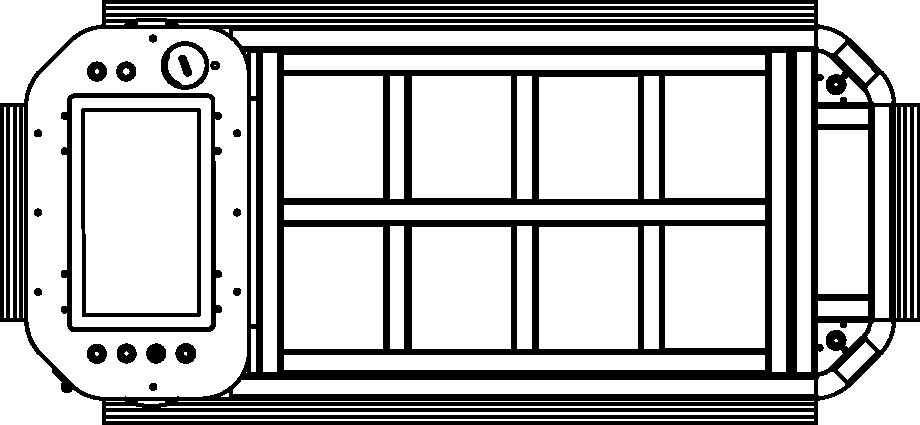
\includegraphics[width=0.9\textwidth]{Bilder/oben.pdf}
			\end{minipage}
			\begin{minipage}[b]{0.49\textwidth}
				(b)
				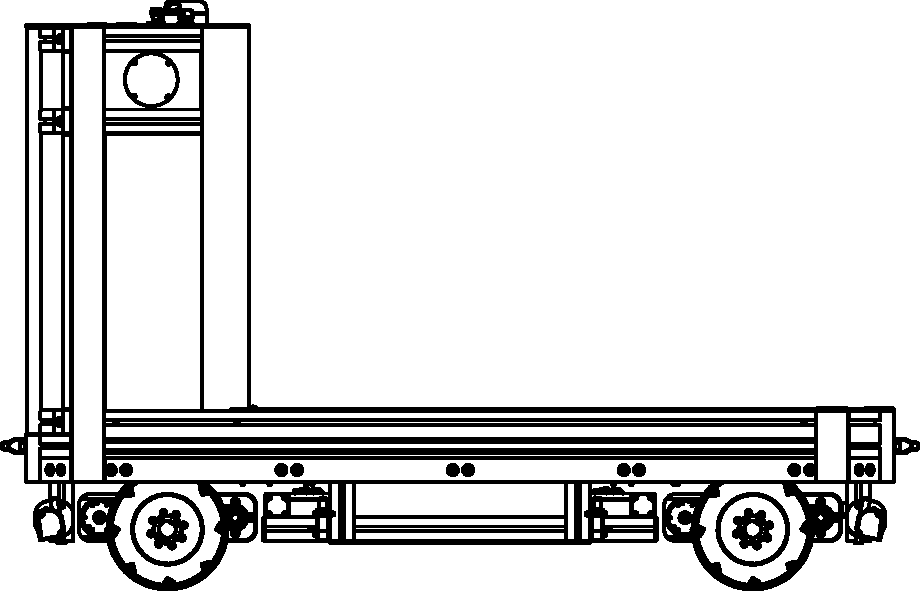
\includegraphics[width=0.9\textwidth]{Bilder/seite.pdf}
			\end{minipage}
			\centering
			\caption{(a) Darstellung des autonomen Logistik-Fahrzeugs aus der Draufsicht. Die acht benachbarten Rechtecke in der Mitte des Fahrzeugs stellen die Ladefläche des Fahrzeugs dar. (b) Darstellung aus der Seitenansicht. Oben links in der Abbildung ist der Schaltschrank zu sehen. Die Räder des Fahrzeugs befinden sich unten links und unten rechts in der Darstellung.}
			\label{fig: Darstellung des ALFs}
		\end{figure}
		
		Das Projekt dieser Masterarbeit wird praktisch am autonomen Logistikfahrzeug angewendet, das aus dem Labor für Antriebstechnik der Hochschule Bochum stammt. Die Idee des ALFs ist es ein Fahrzeug zu entwickeln, das nach seiner Fertigstellung Logistikaufgaben am Standort der Hochschule Bochum lösen soll. Der Entwicklungsprozess stellt sich aus diversen Bachelor- und Masterarbeiten zusammen, die sowohl Hardware, als auch Softwareimplementierungen vorsehen. Bisher wurden zwei Abschlussarbeiten inklusive der praktischen Anwendung am ALF geschrieben. M.Sc. Dennis Hotze und M.Sc. Dominik Eickmann entwickelten in ihrem Masterprojekt das Fahrzeug und konnten Fahraufgaben ferngesteuert und manuell erledigen. Während der darauffolgenden Bachelorarbeit wurde eine Schlupfkompensation entwickelt, die den Drift am Fahrzeug durch Eingabe von Umgebungsinformationen verhindert. Weiterhin wurden Funktionen entwickelt, um grundlegende und autonome Fahraufgaben zu lösen. Das autonome Logistikfahrzeug aus der vorangegangenen Bachelorarbeit dient auch in dieser Masterarbeit als Versuchsplattform. 
	
	\section{Zielsetzung des Projekts}
	\label{sec: Zielsetzung}
		Die Grundidee und Herausforderung des gesamten Masterprojekts, ist eine effektivere und komfortablere Interaktion zwischen Mensch und Roboter. Bisher wurden Zielposen, die im Rahmen einer Fahraufgabe angefahren werden sollten, per Mausklick eingegeben. Fahrmodi mussten manuell am dafür vorgesehenen Controller gewechselt werden. Die Steuerung wird im Zuge der Entwicklung rein optisch und akustisch geschehen, sodass das ALF nicht mehr berührt werden muss. Der akustische Kommunikationsweg wird in der Masterarbeit von Herrn Dittmann behandelt und durch ausgewählte Schnittstellen mit dieser Arbeit verknüpft. Beide Masterarbeiten bilden das vollständige Gesamtsystem. Die optische Komponente der Kommunikation wird im Zuge dieser Masterarbeit behandelt. Ziel ist die Erkennung und Unterscheidung von Personen.
		
		 Dies soll ein Grundstein für zukünftige Projekte am autonomen Logistikfahrzeug darstellen. über Tage hinweg erkannt werden\\
		
		
	